\section{Overview}
In this section we will provide a high-level view and description of the components that our system is made of. The architecture chosen for our system is a three-tier one. The major advantages of this architectural style is the decoupling of the application logic from the presentation logic and the data persistence concerns. Further details about the characteristics of this architectural style will be given in section 2.6, for now we will proceed with the general overview of the system. In the picture below is illustrated a high-level view of the system with an informal notation, where each rectangular box represents a high-level computational unit of the system, meanwhile the double-edged arrow represents 
 the interaction between two components. \\
\begin{figure}[H]
    \centering
    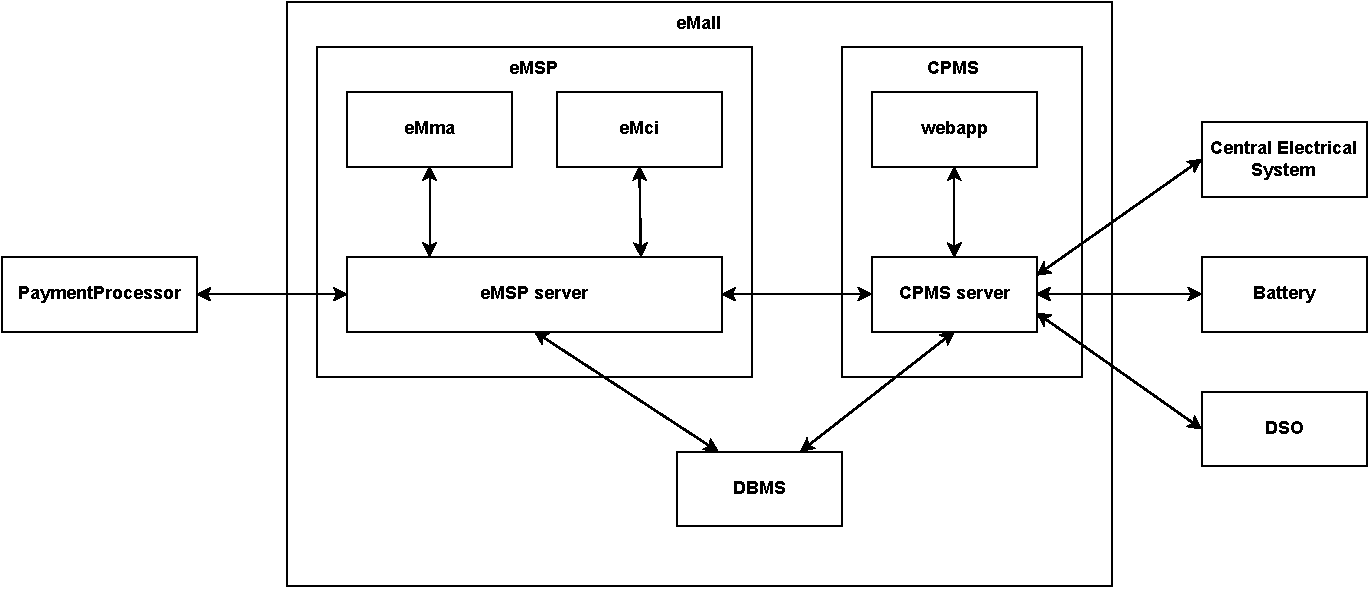
\includegraphics[width=0.8\textwidth]{Images/cp2/overview.pdf}
    \caption{High level description of the components and their interactions}
\end{figure}

\par
%TODO: Bianca please check if you can understand this pargarph
The eMall system, illustrated in the figure, is the objective of this design document. It is clear that the system is divided in two main sub-systems: eMSP and CPMS. This choice is driven by an interoperability requirement of the eMSP and the CPMS with different CPMS and eMSP systems respectively, offered by other companies. Nonetheless, this low-coupling of the CPMS with the eMSP doesn't preclude us from reusing components that have the same functionality in both sub-systems. It is also important to point out that our system, specifically the CPMS sub-system, must be able to interface with the system responsible for managing the technical aspect of the charging point, the system that manages the battery, if present, and the DSO's software system.
\par
As we stated previously, the system has a three-tier architecture. In particular the three tiers are:

\paragraph{Client tier} It's the tier closest to the user and its duty is to manage the user interaction. This means that it must handle the visualization of the content to the user and interpret and translate the user interaction in requests to be forwarded to the application tier. We'd like to remark that this tier doesn't contain any application (or business) logic. We will use a client-side rendering software architecture to design this layer.

\paragraph{Application tier} This is the part where the core and the business logic of the system is implemented, consequently, this second layer realizes the functionalities required to the system, like the booking service or the charging station management service for the CPO. All this functionalities shall be discussed in more detail in the upcoming sections. As we will see in the following section, a micro-services approach has been used to build such layer.

\paragraph{Data tier} The third, and bottom tier, of our system is the data tier, where the persistence concerns of our system are met. The eMall system, both CPMS and eMSP sub-systems, has to handle a large amount of data, which must be carefully stored in order to have a properly working system. The data management is an aspect of software systems that has been thoroughly studied and developed, so the obvious choice for our system is to use an already implemented and tested Database Management System (DBMS).

\section{Component view}
In the section we will discuss and elaborate on the components that compose our system in order to implement the functionalities listed in the RASD document. We will start from a higher level of abstraction to provide a grasp of how the system works, and then we will proceed to further analyze the system at finer levels.
\begin{figure}[H]
    \centering
    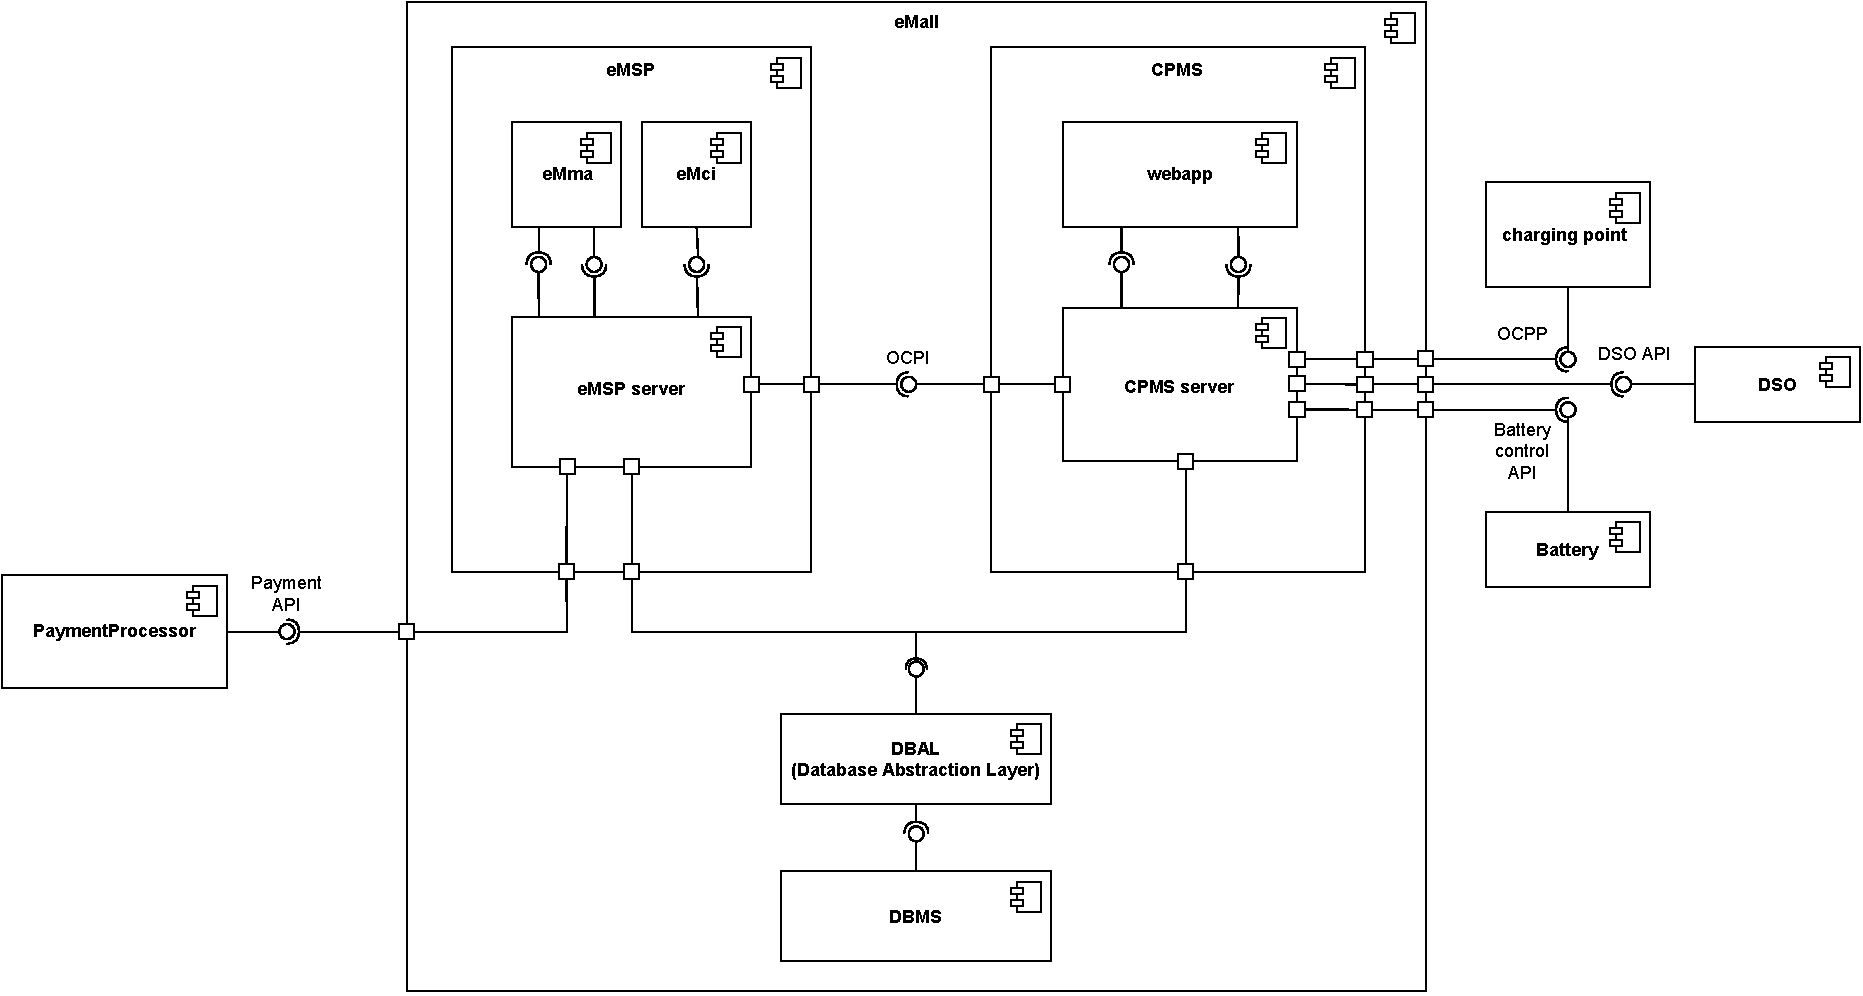
\includegraphics[width=1\textwidth]{Images/cp2/component_overview.pdf}
    \caption{Component view of the system}
\end{figure}
This higher level view of the components gives a simple overview
\begin{figure}[H]
    \centering
    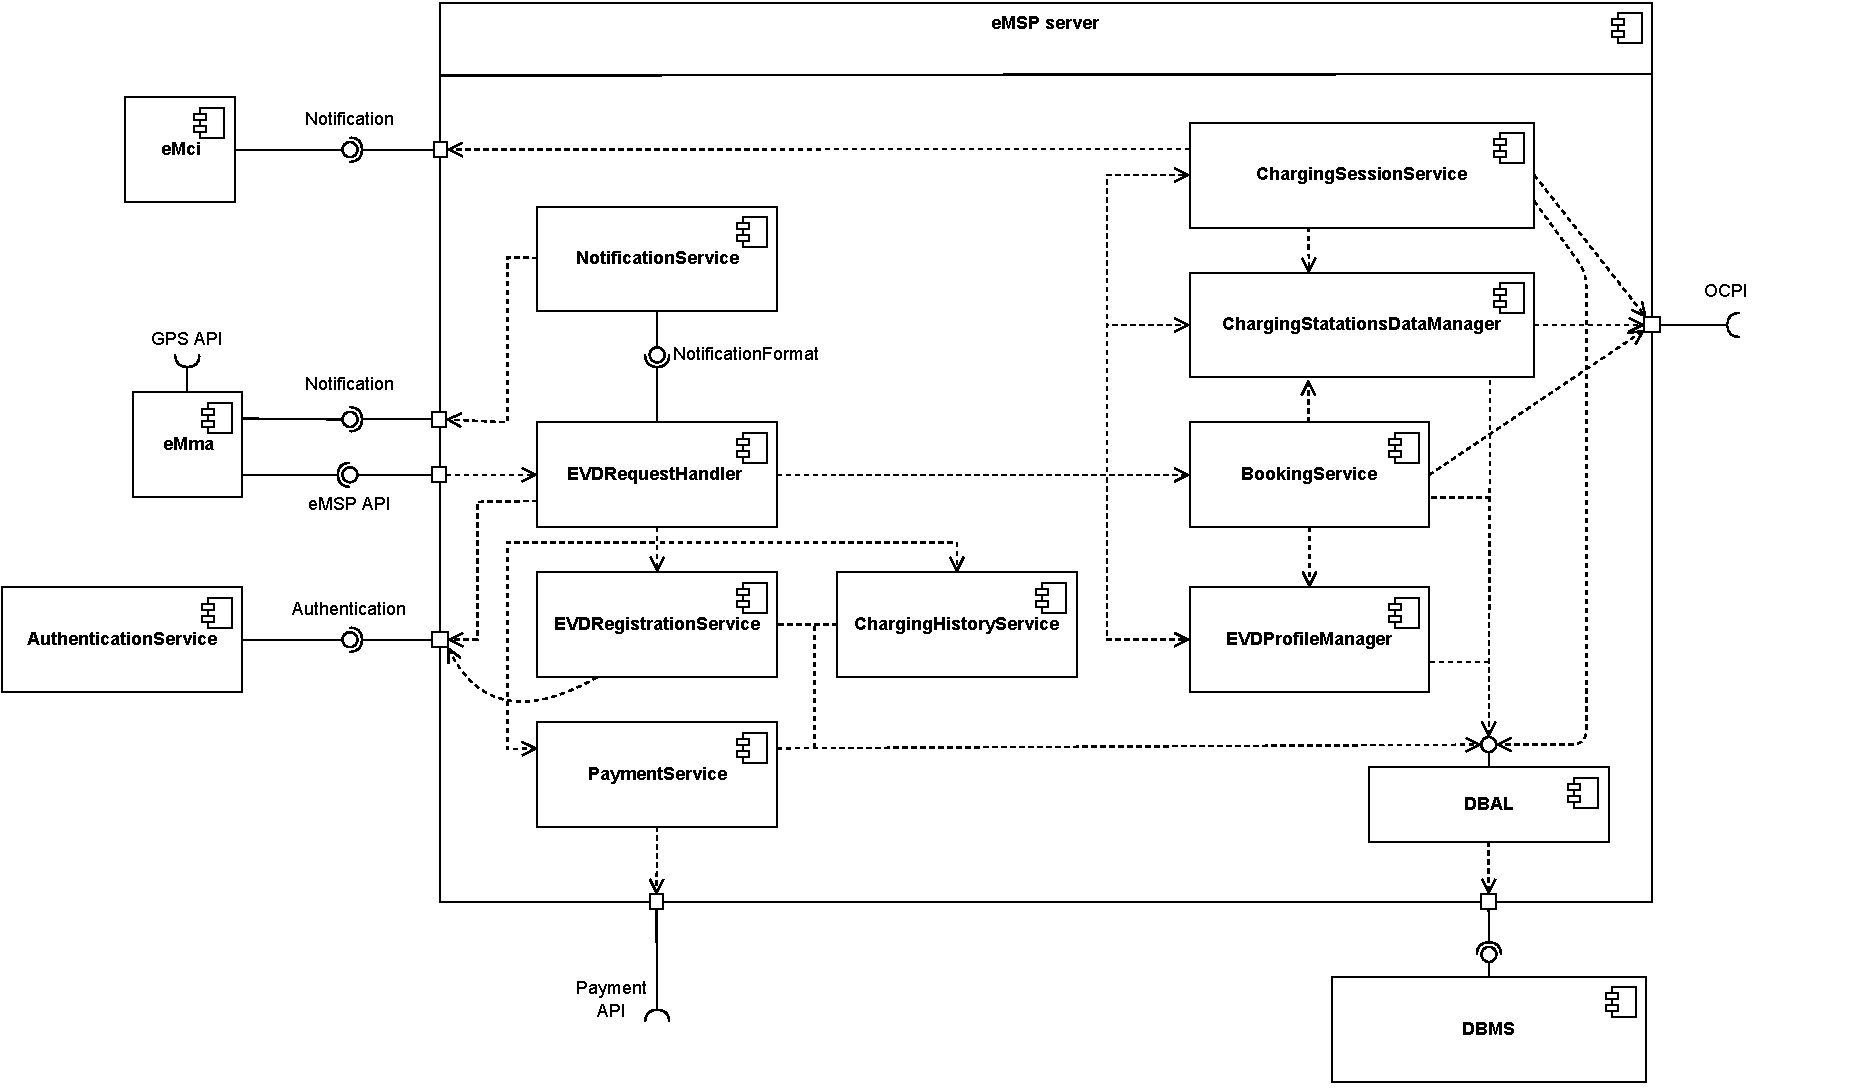
\includegraphics[width=1\textwidth]{Images/cp2/eMSP_server.pdf}
    \caption{eMSP composite structure}
\end{figure}

\begin{figure}[H]
    \centering
    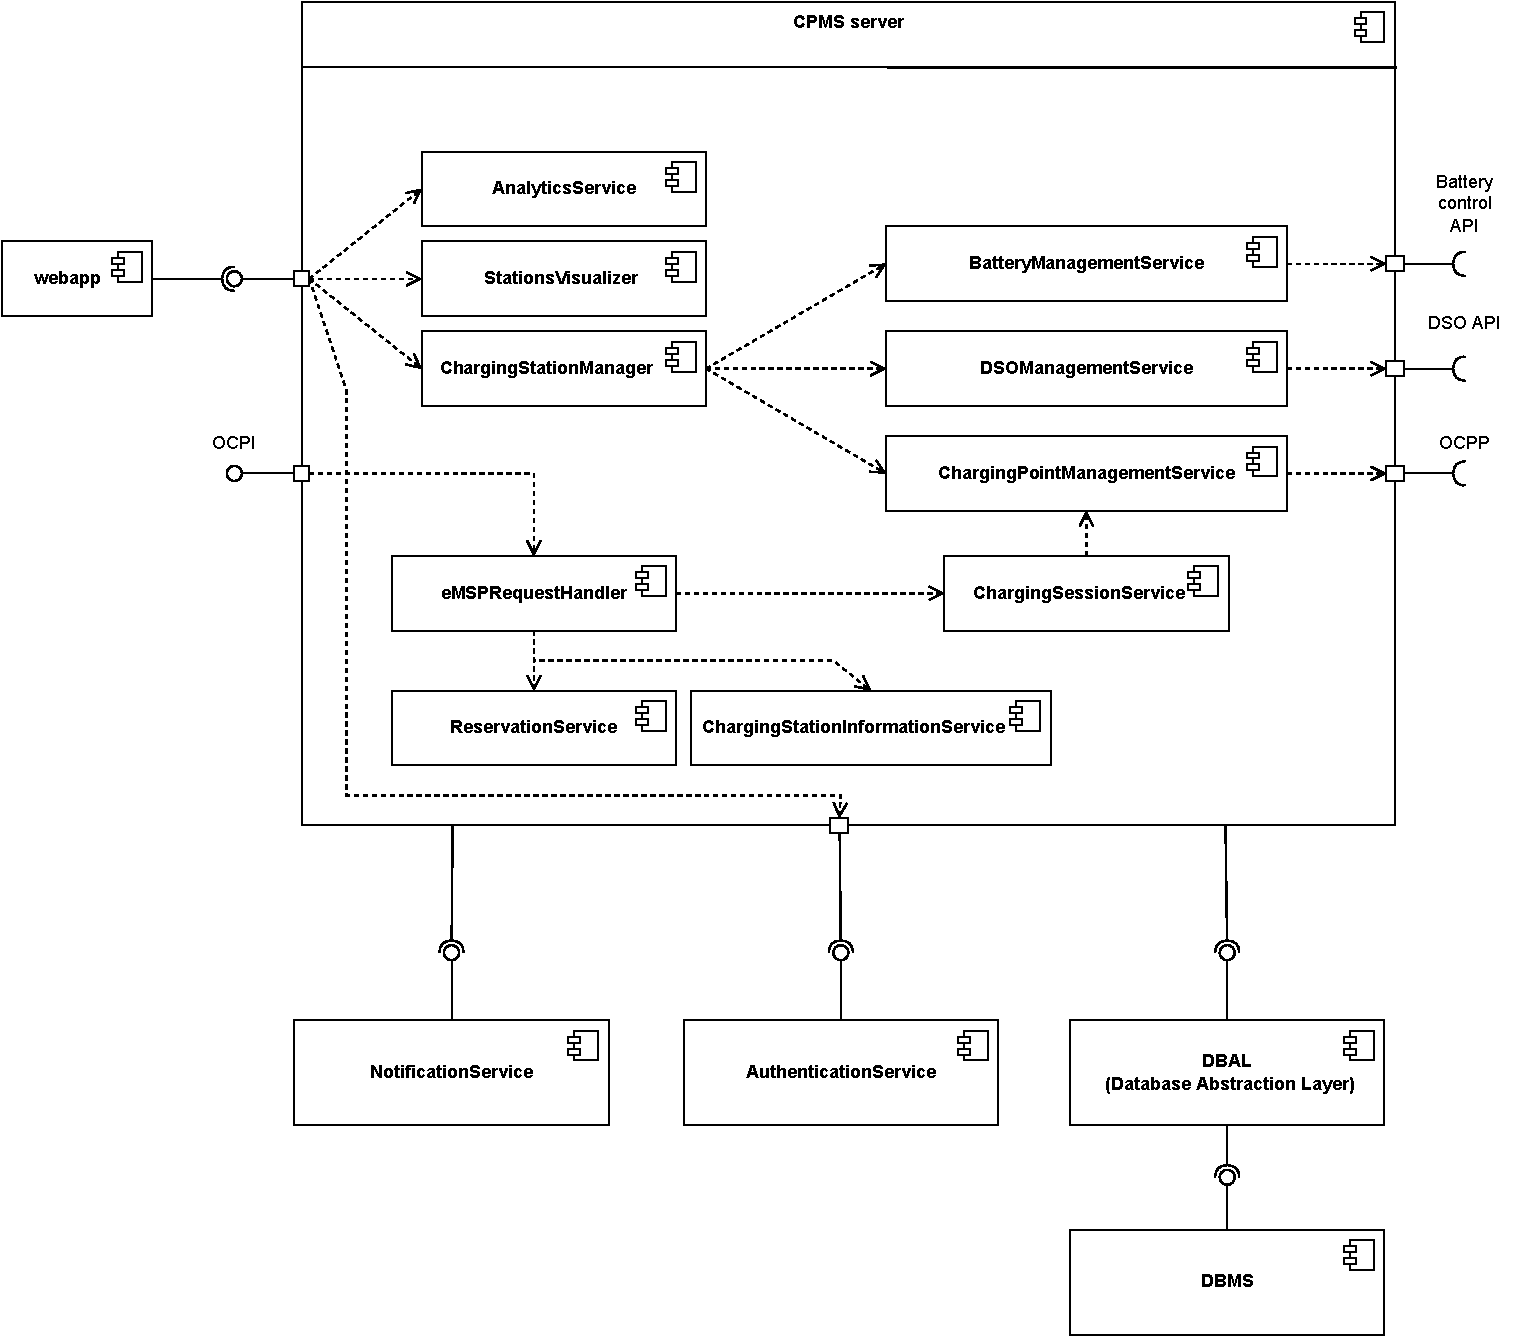
\includegraphics[width=1\textwidth]{Images/cp2/CPMS_server.pdf}
    \caption{CPMS composite structure}
\end{figure}

\section{Deployment view}
\begin{figure}[H]
    \centering
    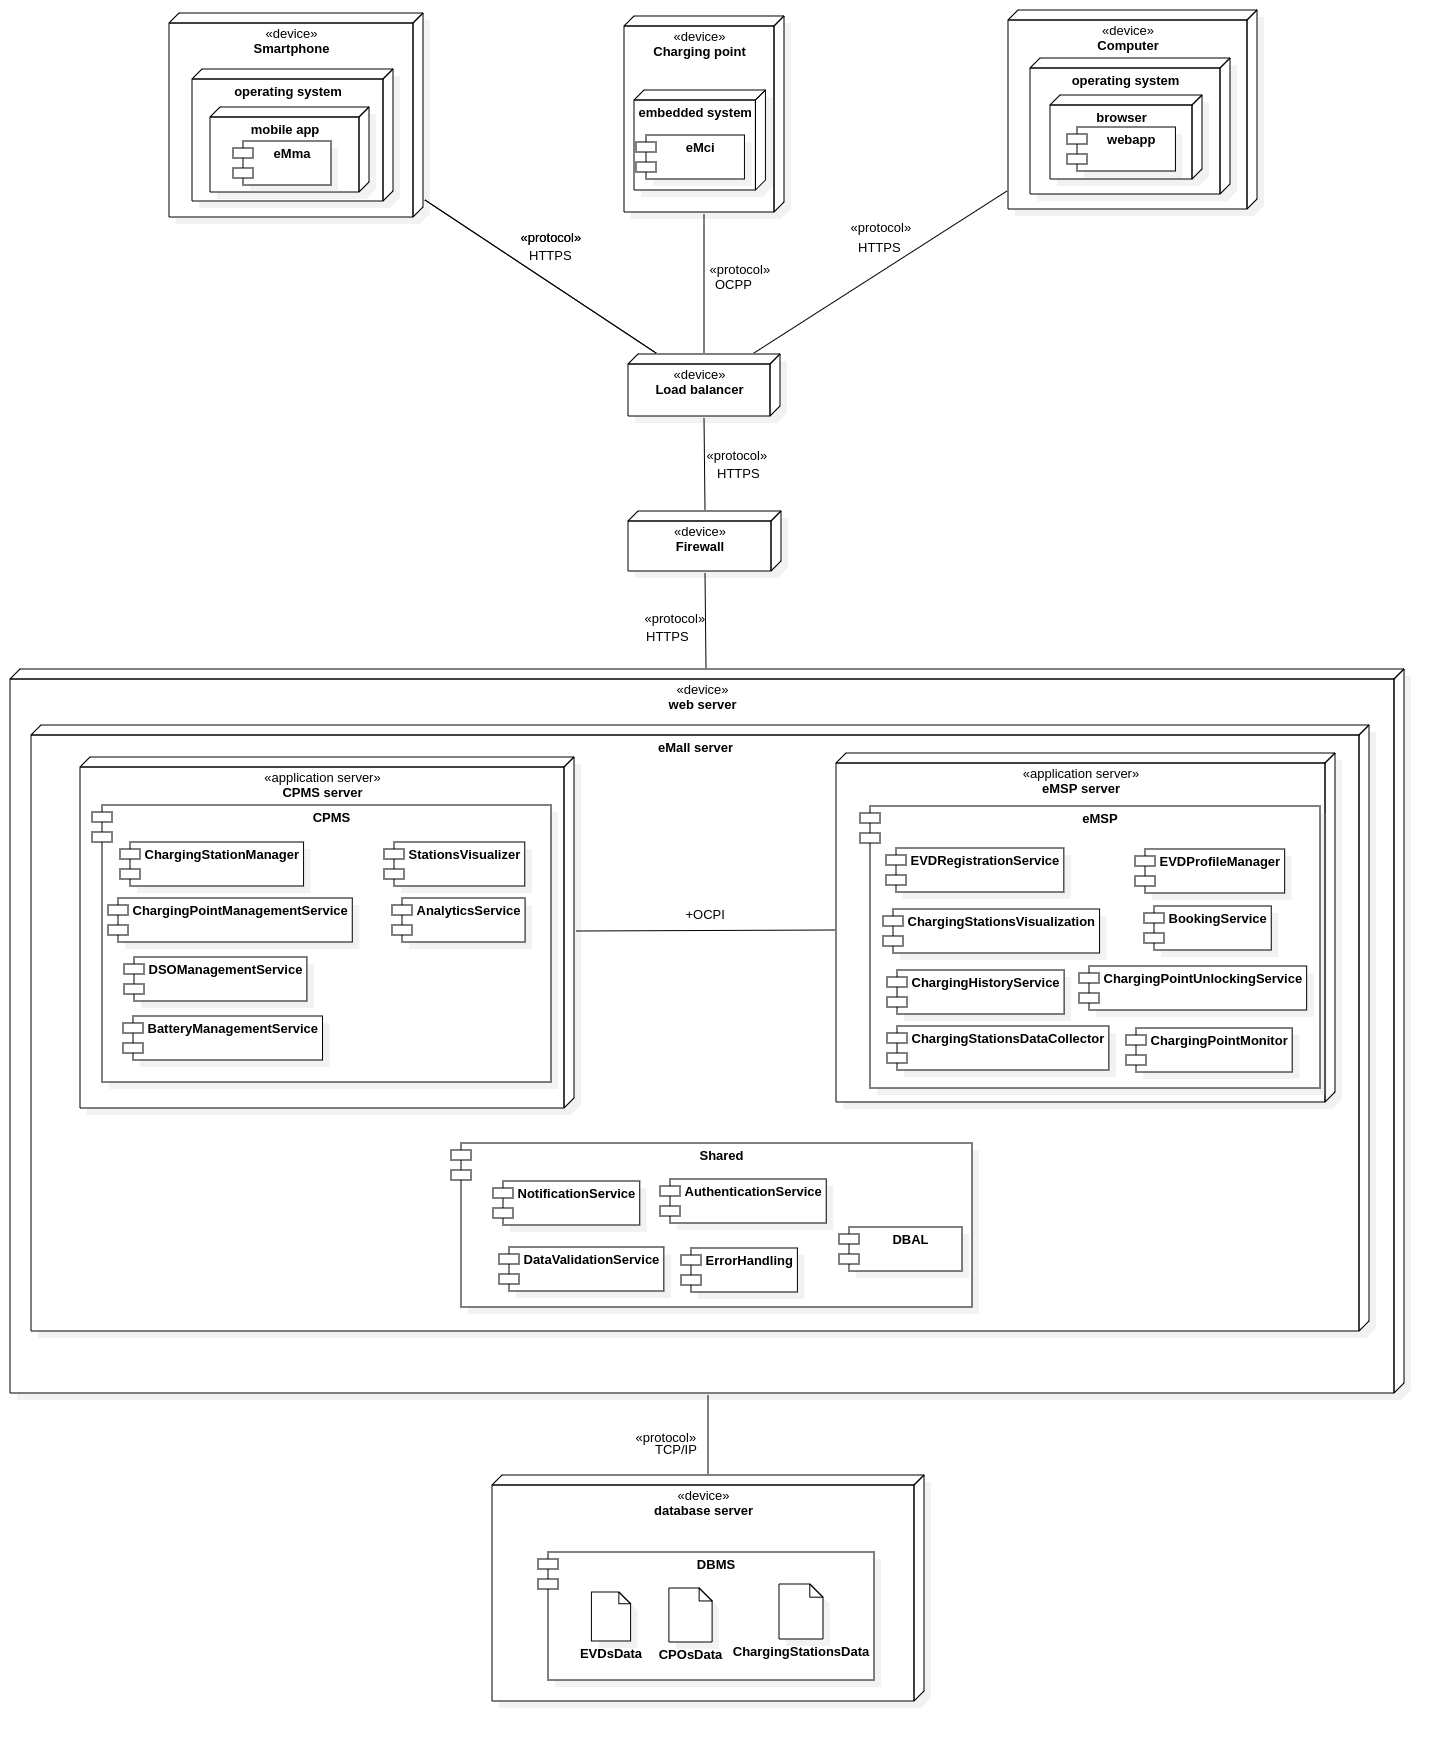
\includegraphics[width=1\textwidth, height=0.9\textheight]{Images/cp2/DeploymentDiagram.png}
    \caption{Deployment view of the system}
\end{figure}
At the client level we can see three different devices interacting with the system:
\begin{itemize}
    \item \textbf{Smartphone} - The smartphone runs the mobile application of the eMall, the eMma, and has internet access in order to send the HTTPS requests to the system. This is the kind of device used by the EVDs that use the eMall
    \item \textbf{Computer} - The computer runs the web application of the eMall, and also has internet access to manage the service through HTTPS requests to the system. This is the kind of device used by the CPOs of the companies that use the eMall to manage their charging stations
    \item \textbf{Charging Point} - The charging point is the specific device used by the EVDs to charge the EVs and it has an embedded system, which through the OCPP protocol communicates with the CPMS part of the eMall system, in order to correctly provide the charging service
\end{itemize}

Between the client level and the application level, we have some architectural elements that allow to achieve some non-functional requirements, such as better performance, scalability, availability and security:
\begin{itemize}
    \item \textbf{Load balancer} - The load balancer is a network device that distributes incoming requests across a group of servers to help improve the performance and availability of the application. A load balancer can help to improve the performance of the application by distributing incoming requests across multiple servers, rather than routing all requests to a single server. This can help to prevent any single server from becoming overloaded, which can improve the overall responsiveness and performance of the application. A load balancer can make it easier to scale the application horizontally by allowing to add or remove servers as needed and this can be useful if we need to add more capacity to handle a growing number of users. A load balancer can, also, help to improve the availability of the application by routing traffic to a healthy server in the event that one of the servers becomes unavailable. We can see that the load balancer is useful to improve different non-functional requirements of the eMall, that can be implemented using different servers to have better characteristics 
    \item \textbf{Firewall} - The firewall allows to protect the network from external threats and unauthorized access, blocking incoming traffic that does not meet the security rules. The firewall is necessary in order to comply with certain regulations and industry standards, because we are handling sensitive data (financial information, personal data), so is necessary to protect the data. The firewall can also help to improve the performance of the application by blocking traffic that is not necessary or relevant to the application, improving the overall responsiveness of the eMall
\end{itemize}

The eMall web application and mobile application provide both static and dynamically generated content, so the system runs web servers for the static content and application servers to generate content dynamically. The load balancer sends to the web server the HTTPS requests that need only static content, and on the other side sends to the correct application server the requests to generate the dynamic content and accomplish more complex functionalities due to the interaction of the eMall components. 
At the application level the deployment diagram shows in a simplistic way the following elements:
\begin{itemize}
    \item \textbf{Web server} - For the web server we have a computer that stores software and website raw data, such as HTML files, images, text documents, and JavaScript files. The hardware of the web server is connected to the web and supports the data exchange with different devices connected to the Internet
    \item \textbf{Application server} - In the deployment diagram on the same hardware we also have the application servers, one for the CPMS and one for the eMSP, with also the shared services. The application servers contain different micro-services, that interact among them and with external APIs, as shown in the previous component diagram. The micro-services could also be implemented on more servers, splitting the eMSP and CPMS application servers in more servers, or creating a redundancy of the available services on different machines to improve performance and availability, exploiting even better the load balancer
    \item \textbf{Shared components} - The shared components shown in the diagram are components that belong to the two application servers, but also to the web server. The web server of the eMall handles part of these functionalities, sending the rest to the application servers  
\end{itemize}

Finally at the lowest level we have the persistent part of the system, which interacts with the eMall trough TCP/IP and is hidden to the higher levels due to the use of the DBAL. The Database level is composed by:
\begin{itemize}
    \item \textbf{Database server} - It hosts the database of the system and manages the different data through a DBMS 
    \item \textbf{Database artifacts} - The different database artifacts shown in the diagram represent physical implementations of the DB, an implementation for the data regarding the EVDs, one for the companies and CPOs data and finally an implementation for the data regarding the charging stations and any other related data
\end{itemize}
For a more secure system we consider not only a DB, but also some replicas, distributed on different machines to guarantee more availability, fault tolerance and disaster recovery. 

\section{Runtime view}

\section{Component interfaces}

\section{Selected architectural styles and patterns}

\section{Other design decisions}